\chapter{Popis a porovnanie súčasných webových technológií}
\label{kapitola2}
Cieľom tejto kapitoly je informovať čitateľa o súčasných webových technológiách. Kapitola obsahuje krátky popis jednotlivých jazykov a technológií, a ich porovnanie. Záver popisuje najpopulárnejšie pomocné webové rámce (ďalej označované ako \texttt{frameworky}) pre vytváranie prezentácií vo webovom prehliadači.

\section{Databáza}
Databáza\cite{database} je množina štrukturovaných údajov ktorá slúži na uloženie informácií. Tieto informácie si môže počítačový program, alebo človek pomocou dopytovacieho jazyka jednoducho získať. 

Aktuálnym najznámejším dopytovacím jazykom je \texttt{SQL}. Počítačový program ktorý slúži na vytváranie dopytov sa nazýva \texttt{Systém riadenia bázy dát}. Štyri základné operácie nad záznamami databáze sa označujú skratkou \texttt{CRUD}, ktorá odpovedá anglickým pojmom v preklade vytvoriť, čítať, upravovať a mazať. 

Rozlišujeme relačné a nerelačné databáze ktoré sú podrobnejšie popísané nižšie.

\subsection{Relačná databáza}
Relačná databáza je typ databáze, ktorá funguje na princípe tabuliek riadkov zoskupených do jednotlivých vzťahov. V relačnej databáze je každý riadok v tabuľke nazývaný ako záznam a každý záznam má pridelený unikátny kľúč \texttt{ID}. Stĺpce tabuľky obsahujú atribúty údajov.

\subsection{Nerelačná databáza}
Nerelačná databáza sa označuje aj ako \texttt{NoSQL}\footnote{\url{https://azure.microsoft.com/cs-cz/overview/nosql-database/}} databáza. Táto technológia je medzi nami už mnohé roky, ale v súčasnej dobe naberá prudký rast popularity kvôli meniacemu sa prostredia údajov. Vývojári sa potrebujú adoptovať, aby si vedeli poradiť so širokou škálou údajov a ich objemom. NoSQL databáze sú efektívne pri spracovaní veľkých objemov vzájomne nesúvisiacich, alebo rýchle sa meniacich údajov s mimoriadnou rýchlosťou dopytov\cite{nosql}. Sú vhodné pre rýchly a flexibilný vývoj aplikácií. Nepoužívajú tabuľkovú schému riadkov a stĺpcov, ale model, ktorý je navrhnutý pre konkrétne požiadavky typu uložených údajov. Na vytvorenie dopytov sa nepoužíva jazyk \texttt{SQL}, ale iné programovacie jazyky. Údaje sú nezávislé na schéme narozdiel od relačných databáz, kde je schému potrebné udržiavať. Dáta môžu byť uložené ako páry kľúč-hodnota, ako \textit{JSON}\footnote{JavaScript Object Notation - spôsob zápisu údajov do objektov} (\textit{JavaScriptový objektový zápis}) dokumenty, ako stĺpce alebo ako graf skladajúci sa z uzlov a hrán. Ich rozdiel je znázornený na obrázku \ref{pic:nosql_types}. V tejto práci sa používa dokumentová databáza \texttt{MongoDB}, jej podrobnejší popis sa nachádza v sekcii \ref{mongodb}.

    \begin{figure}[!hbt]
        \centering
        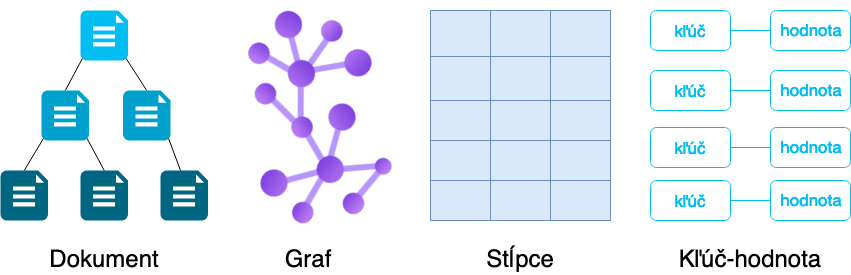
\includegraphics[scale=0.45]{obrazky/nosql_types.png}
        \caption{Ilustrácia typov NoSQL databáz \cite{nosql}.}
        \label{pic:nosql_types}
    \end{figure}

\section{Frontend}
Frontend, alebo častokrát nazývaný aj ako klient, je prezentačná vrstva aplikácie ktorá poskytuje používateľské rozhranie. Je to časť ktorú užívateľ vidí, s ktorou pracuje a ovláda. Medzi najpopulárnejšie technológie pre vývoj frontendu patrí HTML, CSS a JavaScript, pomocou ktorých je táto aplikácia implementovaná. 

\subsection{JavaScript}
JavaScript je objektovo orientovaný skriptovací jazyk. Najviac sa používa pri vývoji dynamických webových aplikácií, ale využíva sa aj pri tvorbe multiplatformových stolových aplikácií a hybridných mobilných aplikácií. Poskytuje interaktivitu nad obsahom. 

Medzi jeho výhody patrí dynamické načítanie stránky, zmena obsahu bez fyzického znova načítania stránky a jeho rozšíriteľnosť. JavaScript sa hlavne zameriaval na klientskú časť aplikácie, kým nenastúpil na scénu framework \texttt{Node.js}(\ref{node}) a podobné serverové technológie, účelom ktorých je tvorba serverovej časti aplikácie.

Existuje niekoľko JavaScriptových frameworkov pre uľahčenie vývoja, pomocou ktorých sa vyhneme takzvaným biolerplate\footnote{Biolerplate - kód ktorý sa musí opakovane vyskytovať na viacerých miestach bez významnej zmeny} kódom. Medzi najpopulárnejšie frameworky patrí Vue.js, React, Angular a Node.js.

\subsection{Vue.js}
Vue.js\cite{vue-guide} je JavaScriptový framework, ktorý patrí medzi najpopulárnejšie nástroje pre tvorbu jednostránkových aplikácii. Je výkonný, rýchly a minimalistický. Stal sa jedným z obľúbených kvôli jeho jednoduchosti. Má veľmi prehľadnú a pestrú dokumentáciu v anglickom aj čínskom jazyku.

Framework bol vytvorený Evanom Youom, ktorý pracoval v Googli a Meteore. V Googli začal používať framework AngularJS, ktorý mu avšak nevyhovoval kvôli jeho striktnému písaniu kódu. Jeho motiváciou bolo vziať najlepšie vlastnosti Angularu a vytvoriť z nich nástroj, ktorý mu zjednoduší a zefektívni prácu.

Frontend aplikácie je implementovaný pomocou tohto frameworku. V sekcii \ref{vue} sa nachádza hlbší a podrobnejší popis jednotlivých vlastností frameworku.

\subsection{Angular}
Angular\cite{angular} je JavaScriptový open-source framework, vytvorený spoločnostou Google. Súčasná verzia sa označuje aj ako Angular 2+, ktorá má zatiaľ jedenásť podverzií. Angular funguje na báze TypeScriptu o ktorom si povieme viac v kapitole \ref{typescript}.

\subsection{React}
React je frontendová JavaScriptová open-source\footnote{Open-source software má dostupný zdrojový kód pre verejnosť} knižnica pre tvorbu užívateľských rozhraní. Na rozdiel od podobných frameworkov ako je Angular, React\cite{react} sa sústreďuje iba na jednu špecifickú oblasť \texttt{MVC}\footnote{Model-View-Controller - softwarová architektúra, ktorá rozdeľuje aplikáciu na dátový model, užívateľské rozhranie a logiku} architektúry, a to je vrstva pohľadu (anglicky \texttt{view}). Knižnica bola predstavená v roku 2013 spoločnosťou Facebook, ktorá ju už niekoľko rokov pred tým používala a vyvíjala. 

\section{Backend}
Backend, mnohokrát nazývaný aj ako server, je základom aplikácie. Tvorí časť, ktorá je skrytá pred používateľom. Jeho úlohou je prijímanie a posielanie dát pre klienta cez aplikačné rozhranie. Tieto údaje spracuje, ukladá, alebo modifikuje v databáze.

\subsection{Node.js}
Node.js\cite{nodejs} je spúšťacie prostredie(runtime environment) pre aplikácie napísané v jazyku JavaScript, mimo webového prehliadača. Je zakladaný na motore Chrome V8 JavaScript, čo znamená že sa prostredie správa rovnako ako webový prehliadač Google Chrome. Node.js sa najčastejšia využíva pri tvorbe serverovej časti webových aplikácií.

Platforma obsahuje viacero frameworkov pre uľahčenie vývoja aplikácií, najpopulárnejším z nich je \texttt{Express.js}, pomocou ktorého je implementovaná serverová časť aplikácie. Podrobnejší popis vlastností oboch technológií sa nachádza v sekcii \ref{node}.

\subsection{Firebase}
Firebase\cite{firebase} je platforma typu \textit{backend-ako-služba} (anglicky \texttt{Backend-as-a-Service}) , ktorá bola vytvorená v roku 2011. V roku 2014 bola odkúpená spoločnosťou Google, ktorá ju doteraz vyvíja. Platforma pomáha v tvorbe, vylepšovaní a škálovaní aplikácií.

BaaS je typ cloudových služieb pre tvorbu aplikácií bez investovania do vlastnej backend infraštruktúry. Uľahčuje vývojárom prácu zapúzdrením služieb na backendu, aby sa mohli sústrediť hlavne na tvorbu frontendu. Medzi tieto služby patrí autentifikácia užívateľov, manažment databáze, monitorovanie a analýza, vzdialené aktualizácie, cloudové úložisko alebo hosting. Všetky tieto služby Firebase poskytuje. 

\subsection{PHP}
Hypertextový preprocessor\cite{php}, v skratke PHP, je populárny skriptovací jazyk, ktorý beží na strane servera. Slúži na vytváranie statických aj dynamických web stránok a aplikácií. Jazyk je bezplatný a použiteľný medzi viacerými platformami. Na PHP sa zakladá viacero frameworkov, ktoré poskytujú základnú štruktúru pre zjednodušený a zrýchlený vývoj. Medzi najpopulárnejšie patria Laravel a Symfony.

Laravel je najpopulárnejší webový PHP framework. Jeho použitie je bezplatné a má voľne dostupný zdrojový kód pre verejnosť. Laravel sa stal obľúbeným kvôli jeho rýchlosti a jednoduchosti. Umožňuje vytváranie komplexných webových aplikácií, bez ohľadu na ich rozsiahlosť. Podporuje MVC architektúru, poskytuje smerovanie, autentifikáciu užívateľov, a mnoho ďalších\cite{php}.

Symfony je jeden z najstarších a najspoľahlivejších PHP frameworkov. Je výbornou voľbou pre vysoko škálovatelné projekty. S Laravelom majú veľa podobných vlastností. Kým Symfony sa skôr zameriava na pokročilých programátorov, Laravel je jednoduchším pre nových vývojárov\cite{php}.

\subsection{Python}
Python je interpretovaný, objektovo-orientovaný programovací jazyk\cite{python}. Poskytuje dynamické typovanie premenných, ktoré je podrobnejšie rozpísané v sekcii \ref{typescript}, a rýchly vývoj aplikácií. Python patrí medzi modulárnych jazykov, podporuje moduly a balíky pomocou ktorých umožňuje znovupoužitie zdrojového kódu. Jazyk obsahuje viacero frameworkov, jedným z najpopulárnejších je Django.

Django je open-source webový framework pre vytváranie webových aplikácií. Je postavaný na princípe MTV (Model-Template-View). Obsahuje dátový model a pohľad ktorý je posielaný do šablóny. Namiesto písaní SQL dotazov preferuje prístup ORM\footnote{ORM - Objektové relačné mapovanie}, transformáciu Python objektov na dotazy.

\section{Nástroje pre tvorbu prezentácií}
Nástroje pre tvorbu prezentácií, ďalej označované ako slideshow frameworky, sú pomôcky pre vytváranie prezentácií vo webovom prehliadači pomocou webových technológií, ako HTML, CSS a JavaScript.

\subsection{Reveal.js}
Reveal.js je najpopulárnejším nástrojom pre tvorbu prezentácií v prehliadači pomocou webových technológií. Framework je založený na čistom JavaScripte a nevyžaduje žiadny iný framework pre jeho použitie. Zdrojový kód projektu je voľne dostupný pre verejnosť. 

Prezentovanie prezentácií v tejto práci sa rieši práve cez tento nástroj, jeho podrobnejší popis a príklad použitia sa nachádza v sekcii \ref{reveal}.

\subsection{Eagle.js}
Eagle.js\footnote{\url{https://github.com/zulko/eagle.js/}} je slideshow framework založený na Vue.js. Podporuje animácie a motívy. Poskytuje užívateľom zopár komunitou vytvorených šablónov pre rýchlejšiu tvorbu prezentácií. 

Nevýhodou Eagle.js je, že jeho vývoj je zanedbaný. Posledná aktualizácia bola vydaná 23.10.2019. Framework používa takzvané mixiny, ktoré sú už v najnovšej verzii Vue.js neschválené (anglicky deprecated) a nahradené \texttt{Composition API}. O mixinoch a Composition API sa čitateľ dozvie viac v sekcii \ref{compositionapi}.

\subsection{Impress.js}
Impress.js\footnote{\url{https://impress.js.org/}} je určený hlavne pre upútanie pozornosti pomocou pestrých animácií. Silnou stránkou tohto frameworku sú animácie poskytované CSS3. Nástroj je vhodný pre prezentácie s malým obsahom.
